\documentclass[12pt]{article}
\usepackage{mathtools,amssymb, amsthm, tikz}
\usetikzlibrary{angles, quotes}
\usepackage[margin=1in]{geometry}
\usepackage[T1]{fontenc}
\usepackage[utf8]{inputenc}
\usepackage{lmodern}
\usepackage{fontspec}
\setmainfont{Times New Roman}

\title{Camera obscura modell}
\author{Pintér Bálint}

\begin{document}
\maketitle
\newpage
\section{Camera obscura modell}
A camera obscuranak (lyukkamera) adott három tulajdonsága a fókusztávolság,
film szélessége és magassága. \\ A film az, amire érkezik a fény és lesz rajta
a kép.\\
\begin{center}
    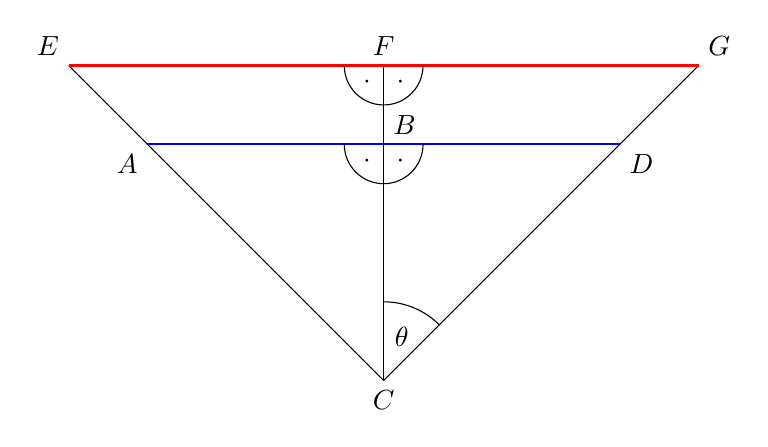
\begin{tikzpicture}
        \coordinate (A) at (0,3);
        \coordinate (B) at (3,3);
        \coordinate (C) at (3,0);
        \coordinate (D) at (6,3);
        \coordinate (E) at (-1,4);
        \coordinate (F) at (3,4);
        \coordinate (G) at (7,4);

        \draw (C) -- (E);
        \draw (C) -- (G);
        \draw (C) -- (F);
        \draw[red, thick] (G) -- (E);
        \draw[blue, thick] (A) -- (D);
        \pic ["$\cdot$", draw=black, angle radius=5mm] {angle = C--B--D};
        \draw pic ["$\cdot$", draw=black, angle radius=5mm] {angle = A--B--C};
        \draw pic ["$\cdot$", draw=black, angle radius=5mm] {angle = E--F--B};
        \draw pic ["$\cdot$", draw=black, angle radius=5mm] {angle = B--F--G};
        \draw pic ["$\theta$", draw=black, angle radius=1cm] {angle = D--C--B};

        \node[below left] at (A) {$A$};
        \node[above right] at (B) {$B$};
        \node[below] at (C) {$C$};
        \node[below right] at (D) {$D$};
        \node[above left] at (E) {$E$};
        \node[above] at (F) {$F$};
        \node[above right] at (G) {$G$};

    \end{tikzpicture}
    \\
    \textbf{1. Ábra:}\\BF a fókusztávolság,\\BC near clipping plane $\text{Z}_{near}$,\\$\theta$ a vertikális FOV (látómező) fele,\\piros EG a film magassága\\kék AD a vászon magassága
\end{center}
A látómező felének ($\theta$) tangense egyszerű trigonometriával felírható.
\begin{align*}
    \tan(\theta) & =\frac{\text{Szemközti befogó}}{\text{Szomszédos befogó}}      \\
    \tan(\theta) & =\frac{\frac{\text{Film magassága}}{2}}{\text{Fókusztávolság}}
\end{align*}
A vászon teteje így kiszámolható. Az 1. ábrán a BD hossza egyenlő a vászon tetejének koordinátájával.
A teteje így:
\begin{alignat*}{2}
    \tan(\theta) & =\frac{\text{t}}{\text{Z}_{near}}                                                   & \quad & \text{/ }\times\text{Z}_{near}                                                      \\
    \text{t}     & =\tan(\theta)\times\text{Z}_{near}                                                  & \quad & \text{/ }\tan(\theta)=\frac{\frac{\text{Film magassága}}{2}}{\text{Fókusztávolság}} \\
    \text{t}     & =\frac{\frac{\text{Film magassága}}{2}}{\text{Fókusztávolság}}\times\text{Z}_{near} &       &
\end{alignat*}
Mivel a vászon szimmetrikus a vászon alja (\textbf{b}ottom) a tetejének az ellentetje:
\[
    \text{b}=-\text{t}
\]
A jobb oldali (r) határát megkaphatjuk úgy, hogy ha a t-t megszorozzuk a film képarányával.
\begin{alignat*}{2}
    \text{r} & = \text{t}\times\frac{\text{Film szélessége}}{\text{Film magassága}} & \quad & \\
    \text{r} & = (\frac{\frac{\text{Film magassága}}{2}}{\text{Fókusztávolság}}\times\text{Z}_{near})\times\frac{\text{Film szélessége}}{\text{Film magassága}}
\end{alignat*}
Látható, hogy a Film magassága-val lehet majd egyszerűsíteni és meg marad a Film szélessége a számlálóban, ami egyenlő lesz a jobb oldali határával. \\
A bal oldali határát hasonlóan az alsó határhoz megkapjuk, ha vesszük a jobb oldali határ ellentettjét.
\[
    \text{b}=-\text{r}
\]
\end{document}